\section{Theory-Matching Experiments}
\label{sec:experiments}

The experiments are controlled diagnostics for the formal claims, not a broad benchmark suite. Each stream is designed so that the Bayes-optimal repair inside an existing atom is different from a refinement that changes the information structure. All learners use a prequential protocol: predict first, observe the consequence, then update. The implementation and generated artifacts are in \path{experiments/run_refinement_theory_experiments.py} and \path{experiments/refinement_theory_results}.

\subsection{Known Bayes-gap calibration}

The first experiment tests the numerical prediction of the repair-only lower bound. We sample
\[
Z\sim \mathrm{Unif}\{1,\ldots,K\},\qquad U\sim \mathrm{Bernoulli}(1/2),
\]
and the old partition observes only $Z$, while the refined partition observes $(Z,U)$. Consequences follow
\[
Y\mid Z=z,U=u\sim \mathrm{Bernoulli}(p_{z,u}),\qquad
p_{z,0}=0.5-\delta,\quad p_{z,1}=0.5+\delta .
\]
Thus $P(Y=1\mid Z=z)=0.5$, so the old atom has log-risk $\log 2$, while the refined risk is $H(0.5+\delta)$. The predicted slope of repair-only cumulative regret is therefore
\[
\Delta_{\mathrm{theory}}=\log 2-H(0.5+\delta)=I(Y;U\mid Z).
\]
We compare smoothed count predictors for the old and refined partitions, plus a one-bit DGM count learner whose candidate distinction is either the true bit $U$ or an independent noise bit.

\begin{figure}[t]
\centering
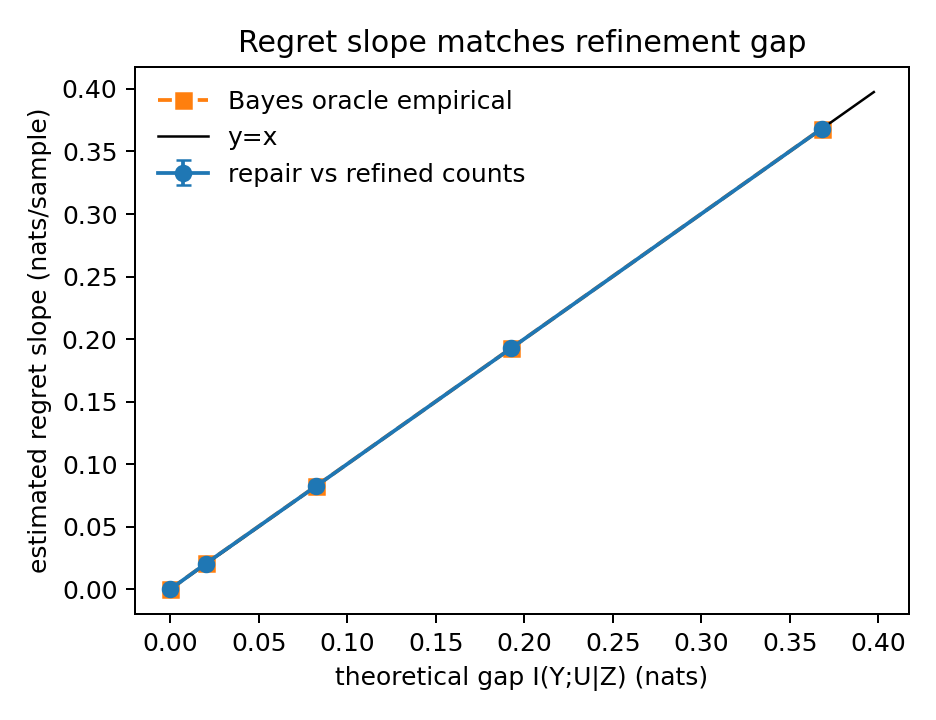
\includegraphics[width=0.62\linewidth]{experiments/refinement_theory_results/bayes_gap_slope_vs_theory.png}
\caption{Known Bayes-gap calibration. The estimated repair-only regret slope matches the theoretical refinement gap $I(Y;U\mid Z)$ under log loss.}
\label{fig:bayes-gap-slope}
\end{figure}

\begin{table}[t]
\centering
\small
\begin{tabular}{ccccc}
\toprule
$\delta$ & Theory gap & Repair/refined slope & Bayes-oracle slope & Accepted noise splits \\
\midrule
$0.0$ & $0.0000$ & $-0.0000\pm0.0000$ & $0.0000\pm0.0000$ & $0.00$ \\
$0.1$ & $0.0201$ & $0.0206\pm0.0013$ & $0.0206\pm0.0013$ & $0.00$ \\
$0.2$ & $0.0823$ & $0.0824\pm0.0012$ & $0.0824\pm0.0012$ & $0.00$ \\
$0.3$ & $0.1927$ & $0.1928\pm0.0041$ & $0.1929\pm0.0041$ & $0.00$ \\
$0.4$ & $0.3681$ & $0.3682\pm0.0037$ & $0.3682\pm0.0038$ & $0.00$ \\
\bottomrule
\end{tabular}
\caption{Regret-slope calibration over 16 seeds. Slopes are in nats per sample, estimated from the second half of each stream. At $\delta=0$, $U$ carries no consequence information and no refinement is accepted.}
\label{tab:bayes-gap-calibration}
\end{table}

The agreement is the important point: the error made by repair-only counts is not an optimizer artifact. Its asymptotic slope is the information-structure gap predicted by the theorem. The $\delta=0$ row is the corresponding negative control.

\subsection{Guarded refine-or-repair decisions}

The second experiment tests whether refinement is consequence-sensitive rather than novelty-sensitive. We create two old atoms. In the repair atom, $Y\sim\mathrm{Bernoulli}(0.8)$ and all candidate distinctions are independent of $Y$, but the current local prediction is deliberately stale at $q(Y=1)=0.2$. The correct action is repair. In the refinement atom, $Y\mid U=0\sim\mathrm{Bernoulli}(0.1)$ and $Y\mid U=1\sim\mathrm{Bernoulli}(0.9)$, so the correct action is to refine by $U$.

The candidate pool contains the true distinction $U$, twenty independent noise bits, and six geometry-only bits that are visually separable but independent of $Y$. Candidate proposal and validation use separate buffers. A refinement is accepted only when its penalized held-out gain exceeds both zero and the held-out repair gain by a margin.

\begin{table}[t]
\centering
\small
\begin{tabular}{ccccc}
\toprule
Scoring buffer & True recall & False refinement & Spurious acceptance & Repair accuracy \\
\midrule
$32$ & $0.956$ & $0.001$ & $0.001$ & $0.999$ \\
$64$ & $0.991$ & $0.000$ & $0.000$ & $1.000$ \\
$128$ & $1.000$ & $0.000$ & $0.000$ & $1.000$ \\
$256$ & $1.000$ & $0.000$ & $0.000$ & $1.000$ \\
$512$ & $1.000$ & $0.000$ & $0.000$ & $1.000$ \\
\bottomrule
\end{tabular}
\caption{Guarded refinement decisions over 800 trials per cell type and buffer size. The learner accepts the consequence-useful distinction and rejects noise or geometry-only distinctions.}
\label{tab:guarded-refinement}
\end{table}

\begin{figure}[t]
\centering
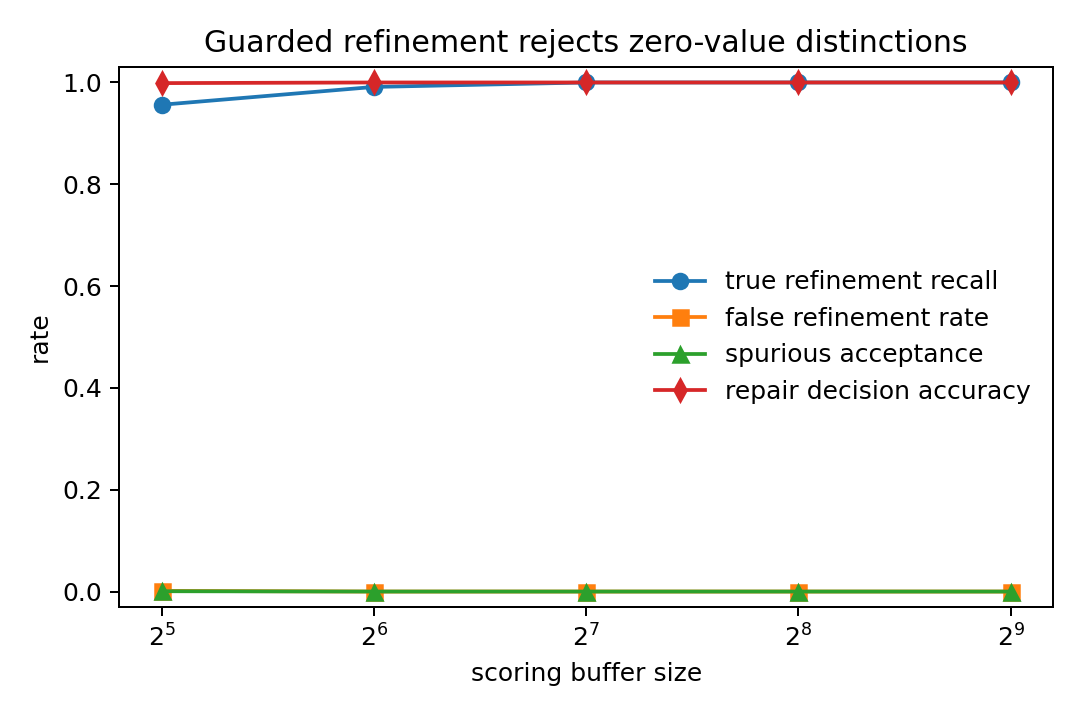
\includegraphics[width=0.62\linewidth]{experiments/refinement_theory_results/guarded_sample_size_curve.png}
\caption{Sample-size curve for the guarded decision rule. Larger scoring buffers preserve true-refinement recall while driving false refinement and spurious acceptance to zero.}
\label{fig:guarded-refinement}
\end{figure}

This directly probes the algorithmic distinction between ``new feature'' and ``useful refinement.'' The repair atom contains a large empirical repair gain and many possible bits, but no bit has stable consequence value, so the guarded rule repairs instead of growing the graph.

\subsection{Graph-memory ablation on contextual XOR}

The third experiment checks the data-structure claim. The stream is a contextual XOR problem: $Y=b_1\oplus b_2\oplus c$, where the initial atoms are keyed by the two visible signs $(b_1,b_2)$ and the useful edge-generated distinction is the context bit $c$. We add nuisance coordinates so that prototype growth and cache baselines can create geometrically distinct states without obtaining the consequence-relevant partition.

\begin{table}[t]
\centering
\scriptsize
\setlength{\tabcolsep}{3pt}
\resizebox{\linewidth}{!}{%
\begin{tabular}{lcccccc}
\toprule
Model & Preq. acc. & Preq. NLL & Test acc. & Concepts & Context edges & Purity \\
\midrule
Full DGM refine+repair+edges & $\mathbf{0.959\pm0.002}$ & $\mathbf{0.073}$ & $\mathbf{0.998}$ & $8.0$ & $4.0$ & $0.997$ \\
DGM repair only & $0.503\pm0.007$ & $0.696$ & $0.502$ & $4.0$ & $0.0$ & $0.514$ \\
DGM refine only, no repair & $0.501\pm0.007$ & $0.693$ & $0.496$ & $8.0$ & $4.0$ & $0.997$ \\
No-edge centroid growth & $0.504\pm0.004$ & $0.698$ & $0.502$ & $8.0$ & -- & $0.155$ \\
$k$NN/cache, same budget & $0.497\pm0.006$ & $0.785$ & $0.499$ & $8.0$ & -- & -- \\
$k$NN/cache, larger budget & $0.494\pm0.005$ & $0.788$ & $0.498$ & $64.0$ & -- & -- \\
\bottomrule
\end{tabular}
}
\caption{Contextual XOR graph-memory ablation over 10 seeds. Full DGM accepts all four context edges and no spurious edges. Repair-only cannot separate incompatible consequences; refine-only recovers the structure but has no local memory repair; no-edge and cache baselines do not recover the consequence partition under the same stream.}
\label{tab:contextual-xor-ablation}
\end{table}

This separates the two mechanisms. Refine-only recovers the right partition structure, as shown by high purity, but without local memory repair its predictions remain at chance. Repair-only has local counts but the wrong atoms. The full graph-memory learner combines edge-generated refinement with local repair and uses only the eight target concepts rather than relying on unbounded growth.

\paragraph{Scope.}
These experiments do not claim that DGM is a finished competitive language-modeling system. They test the mechanisms required by the theory: repair-only regret has the predicted information-structure slope; the refinement rule accepts only consequence-useful distinctions; and graph-generated refinement plus local repair is more effective than either operation alone.
